\chapter{Circular Motion and Orbits}
	\section{Centripetal Forces and Accelerations}
	\subsection{Centripetal Force} \index{Force, Centripetal}
	We have already learned that an object in motion will continue to move in a straight line, assuming no forces are acting on the object.  In order for an object to move along a circular path, there must therefore be a force acting on the object to keep it from moving in a straight line.  If you whirl a mass on a string around in a circle, tension in the string keeps the mass from continuing to move in a straight line.  As the Moon orbits the Earth, the gravitational attraction between the Moon and the Earth keeps the Moon in its orbit around the Earth.  Any force that keeps an object moving along a circular path is called a \textbf{Centripetal Force} (Centripetal literally translates from Latin as ``center seeking'').  Any centripetal force can be described as:
	
	\begin{mdframed}[backgroundcolor=orange!20!white]
	\begin{equation}
	F_c = \frac{mv^2}{r}
	\label{equation:centripetalforce}
	\end{equation}
		
	\end{mdframed}
	

	The direction of a centripetal force is always toward the center of the circle.  

	
	\subsection{Centripetal Acceleration} \index{Acceleration, Centripetal}
	
	
	
	When an object moves in a circle, even if its speed remains constant, its velocity is constantly changing due to its constant change in direction of motion.  Thus the object must be constantly accelerating in a direction toward the center of the circle.  Using Equation \ref{equation:centripetalforce} and Newton's Second Law, it is possible to prove that centripetal acceleration is given by:			
	\begin{mdframed}[backgroundcolor=orange!20!white]
	\begin{equation}
	a_c = \frac{v^2}{r}
	\end{equation}
	\end{mdframed}
	Just as centripetal force is always directed toward the center of the circle, centripetal acceleration is also always directed toward the center of the circle.  
	
	
	\begin{mdframed}[backgroundcolor=blue!10!white]
		\begin{center}
			\textbf{Example \thesubsection}
		\end{center}
		\textbf{Problem:} A children's toy consists of a 0.5kg ball attached to the end of a light 0.3-meter-long rope.  A child grabs the toy from the end of the rope and swings the ball around in a circle above his head with a tangential speed of 2 m/s.  What is the tension in the rope? 
		
		\vspace{0.1in}
		
		\textbf{Solution:} In order to keep moving in a circle, tension in the rope must act as the centripetal force.  Therefore, the tension in the rope is given by:
	
		\begin{equation*}
			F_T = F_c = \frac{mv^2}{r} = \frac{0.5 kg \cdot (2 m/s )^2}{0.3m} \approx \boxed{6.667 N}
		\end{equation*}
		
		\end{mdframed}
	
	
		\begin{mdframed}[backgroundcolor=blue!10!white]
		\begin{center}
			\textbf{Example \thesubsection.2}
		\end{center}
		\textbf{Problem:} A toy car travels around a loop of diameter 0.3 meters.  What is the minimum speed the car needs to travel in order to make it around the loop?
		
		\vspace{0.1in}
		
		\textbf{Solution:} When the car is traveling around the loop, it is most likely to fall off at the top.  If gravity is stronger than the needed centripetal force, the car falls.  If gravity is equal to, or even less than the required centripetal force, the car stays on the track.  Thus:
		
		\begin{equation*}
		F_g \leq  	F_c 
		\end{equation*}
		Substituting equations shows: 
		\begin{equation*}
		\cancel{m}g \leq  	\frac{\cancel{m}v^2}{r} 
		\end{equation*}
		Solving for v yields: 
		\begin{equation*}
				\sqrt{g r} \leq v
		\end{equation*}
		Note that the diameter is given in the problem, but the formula requires the radius.  Thus, substituting numbers gives: 
				\begin{equation*}
		\sqrt{(9.81 \frac{m}{s^2})(0.15m) } \leq v
		\end{equation*}
		Thus:
				\begin{equation*}
		\boxed{1.213 \frac{m}{s}  \lessapprox v}
		\end{equation*}
		
		
		
	\end{mdframed}
	
	\newpage
	
	\section{Kepler's Laws of Planetary Motion} \index{Kepler's Laws of Planetary Motion} \index{Planetary Motion, Kepler's Laws of}
	\subsection{Kepler's First Law}
	    Kepler's first law states that the orbit of a planet is an ellipse with the Sun at one of the two foci:
	    
	    

		\begin{figure}[H]	    	
	    \begin{center}


 
 
 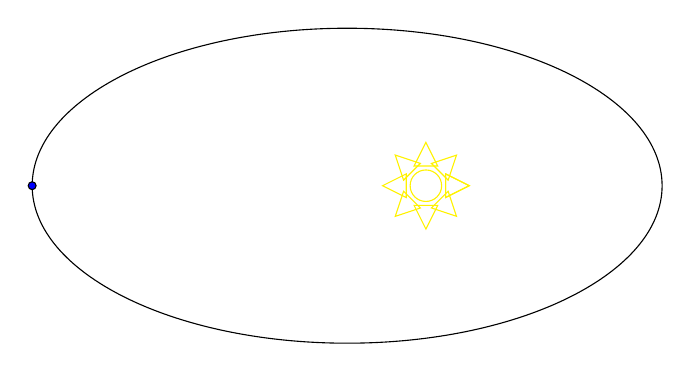
\begin{tikzpicture}[x=0.1cm,y=0.1cm]
 \draw[yellow] (2,0)
 arc (0:360:2);
 \foreach \angle in { 0,45,...,360 }{
 	\draw [yellow,rotate around={\angle:(0,0)}]
 	(2.5,0)    
 	-- +(0,-1.5)
 	-- +(3,0)
 	-- +(0,1.5)
 	-- cycle; }
 
\draw (-10,0) ellipse (4cm and 2cm);
\draw[fill=blue] (-50,0) circle (.5);
 
 
 

	    \end{tikzpicture}
	    \caption{Planets orbit the sun along elliptical path.  This diagram exaggerates the eccentricity of the orbital path to show the placement of the sun.}
    \end{center}
\end{figure}
	    
One should note that most planet's orbital path is much closer to circular than the diagram above.  For instance, here is earth's orbit compared to a perfect circle:


\begin{figure}[H]
\begin{center}
\begin{tabular}{c c}

\begin{tikzpicture}
\draw (0,0) ellipse (2 and 1.98);
\end{tikzpicture}
&
\begin{tikzpicture}
\draw (0,0) circle (2);

\end{tikzpicture}	
\\
Earth's Orbit & Circle
\end{tabular}
\caption{Earth's orbit shape compared to a circle.}
\end{center}
\end{figure}




		The Eccentricity of an ellipse can be found using: 
		
			\begin{mdframed}[backgroundcolor=orange!20!white]
			
			\begin{equation}
			\varepsilon = \sqrt{1-\frac{b^2}{a^2}} 
			\label{equation:eccentricity}
			\end{equation}
		\end{mdframed}
		where a is the semimajor axis and b is the semiminor axis, as shown in the diagram:
		

			\begin{figure}[H]
\begin{center}
	

		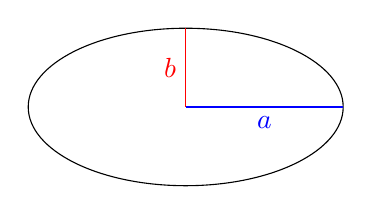
\begin{tikzpicture}
		\draw (0,0) ellipse (2cm and 1cm);
		\draw [blue](0,0) -- (2,0); 
		\draw[red] (0,0) -- (0,1); 
		\node (n1) at (1,0) [below,blue] {$a$};
		\node (n2) at (0,.5) [left,red] {$b$};
		\end{tikzpicture}
		\caption{The semimajor axis ($a$) and semiminor axis ($b$) of an ellipse.}
		\end{center}
		\end{figure}
			
	\subsection{Kepler's Second Law}
		A line segment joining a planet and the Sun sweeps out equal areas during equal intervals of time.
		
		This can be expressed as: 
		
				
		\begin{mdframed}[backgroundcolor=orange!20!white]
			
			\begin{equation}
			\frac{A_1}{t_1} = \frac{A_2}{t_2}
			\label{equation:kep2nd}
			\end{equation}
		\end{mdframed}
		
		It can be shown that this expression is equivalent to:
		
		
					
		\begin{mdframed}[backgroundcolor=orange!20!white]
			
			\begin{equation}
			r_1 v_1 = r_2 v_2
			\label{equation:kep2ndalt}
			\end{equation}
		\end{mdframed}
		Where $r_1$ and {$r_2$} are the average radii for each segment of arc, and $v_1$ and $v_2$ are the average velocities, respectively. 
		
		
		
	\subsection{Kepler's Third Law}
			The square of the orbital period of a planet is directly proportional to the cube of the semi-major axis of its orbit. Thus, for any two planets orbiting the sun, 
			
					\begin{mdframed}[backgroundcolor=orange!20!white]
						\begin{equation}
			\frac{{T_1}^2}{{R_1}^3} = \frac{{T_2}^2}{{R_2}^3}
			\label{equation:kep3rd}
			\end{equation}
		\end{mdframed}
	
	
	
	
	\section{Newton's Law of Universal Gravitation} \index{Universal Gravitation, Law of}
	
	Newton's Law of Universal Gravitation is a way of calculating the gravitational force between any two objects with mass.  It is given by: 
	\begin{mdframed}[backgroundcolor=orange!20!white]
		\begin{center}
\textbf{Newton's Law of Universal Gravtation}
		\end{center}
		\begin{equation}
		F_g = \frac{G m_1m_2}{r^2}
		\label{equation:UniversalGravitation}
		\end{equation}
	\end{mdframed}
	where G is the Universal Gravitational Constant:
	
		\begin{mdframed}[backgroundcolor=green!20!white]
		\begin{equation*}
		G = 6.67 \times 10^{-11} \si{\frac{Nm^2}{kg^2}}
		\label{equation:universalgravconstant}
		\end{equation*}
	\end{mdframed}	
	
	 
	 
	 The masses of the two objects are $m_1$ and $m_2$, and $r$ is the distance between these objects.   
	
	
	Sometimes, you will see equation \ref{equation:UniversalGravitation} written with a negative sign in order to make it consistent with some of the laws of electrostatics, studied in \autoref{chap:Electrostatics}. However, you will likely end up assigning a sign to the force, according to the coordinate system you have defined for the problem. 
	
	
	
	
	
	\section{Orbital Motion} \index{Orbits}
	Whenever a object orbits another that has a much larger mass, if the orbit can be approximated by a circle, the gravitational attraction between the two bodies acts as a centripetal force.  Thus, a fundamental realization of orbital mechanics is:
	

		


	


